\documentclass[a4paper,12pt]{article}

\usepackage{float}


\usepackage[utf8]{inputenc}
\usepackage[dvips]{graphicx}
%\usepackage{a4wide}
\usepackage{epsfig}
\usepackage{fancybox}
\usepackage{verbatim}
\usepackage{array}
\usepackage{latexsym}
\usepackage{alltt}
\usepackage{amssymb}
\usepackage{amsmath,amsthm}
\usepackage{bm}
\usepackage{wasysym}

%\usepackage{fullpage}
%\usepackage{hyperref}
\usepackage{listings}
\usepackage{color}
\usepackage{algorithm}
\usepackage{algpseudocode}
\usepackage[hmargin=2cm,vmargin=3.0cm]{geometry}
%\topmargin=0cm
%\topmargin=-1.8cm
%\addtolength{\textheight}{6.5cm}
%\addtolength{\textwidth}{2.0cm}
%\setlength{\leftmargin}{-3cm}
%\setlength{\oddsidemargin}{0.0cm}
%\setlength{\evensidemargin}{0.0cm}

%misc libraries goes here
\usepackage{tikz}
\usepackage{tikz-qtree}
\usetikzlibrary{automata,positioning}

\usepackage{multicol}
\usepackage{enumitem}

\usepackage[most]{tcolorbox}

\usepackage[colorlinks=true,urlcolor=black,linkcolor=black]{hyperref}


\lstdefinestyle{customtex}{
    %backgroundcolor=\color{lbcolor},
    tabsize=2,
    language=TeX,
    numbers=none,
    basicstyle=\footnotesize\ttfamily,
    numberstyle=\footnotesize,
    aboveskip={0.0\baselineskip},
    belowskip={0.0\baselineskip},
    %
    columns=flexible,
    keepspaces=true,
    fontadjust=true,
    upquote=true,
    %
    breaklines=true,
    prebreak=\raisebox{0ex}[0ex][0ex]{\ensuremath{\hookleftarrow}},
    frame=single,
    showtabs=false,
    showspaces=false,
    showstringspaces=false,
    %
    %identifierstyle=\color[rgb]{0,0.2,0.8},
    identifierstyle=\color[rgb]{0,0,0.5},
    %identifierstyle=\color[rgb]{0.133,0.545,0.133},
    %keywordstyle=\color[rgb]{0.8,0,0},
    %keywordstyle=\color[rgb]{0.133,0.545,0.133},
    keywordstyle=\color[rgb]{0,0,0.5},
    %commentstyle=\color[rgb]{0.133,0.545,0.133},
    commentstyle=\color[rgb]{0.545,0.545,0.545},
    %stringstyle=\color[rgb]{0.827,0.627,0.133},
    stringstyle=\color[rgb]{0.133,0.545,0.133},
    %
    literate={â}{{\^{a}}}1 {Â}{{\^{A}}}1 {ç}{{\c{c}}}1 {Ç}{{\c{C}}}1 {ğ}{{\u{g}}}1 {Ğ}{{\u{G}}}1 {ı}{{\i}}1 {İ}{{\.{I}}}1   {ö}{{\"o}}1 {Ö}{{\"O}}1 {ş}{{\c{s}}}1 {Ş}{{\c{S}}}1 {ü}{{\"u}}1 {Ü}{{\"U}}1 {~}{$\sim$}{1}
}

\lstdefinestyle{output}{
    %backgroundcolor=\color{lbcolor},
    tabsize=2,
    numbers=none,
    basicstyle=\footnotesize\ttfamily,
    numberstyle=\footnotesize,
    aboveskip={0.0\baselineskip},
    belowskip={0.0\baselineskip},
    %
    columns=flexible,
    keepspaces=true,
    fontadjust=true,
    upquote=true,
    %
    breaklines=true,
    prebreak=\raisebox{0ex}[0ex][0ex]{\ensuremath{\hookleftarrow}},
    frame=single,
    showtabs=false,
    showspaces=false,
    showstringspaces=false,
    %
    %identifierstyle=\color[rgb]{0.44,0.12,0.1},
    identifierstyle=\color[rgb]{0,0,0},
    keywordstyle=\color[rgb]{0,0,0},
    commentstyle=\color[rgb]{0,0,0},
    stringstyle=\color[rgb]{0,0,0},
    %
    literate={â}{{\^{a}}}1 {Â}{{\^{A}}}1 {ç}{{\c{c}}}1 {Ç}{{\c{C}}}1 {ğ}{{\u{g}}}1 {Ğ}{{\u{G}}}1 {ı}{{\i}}1 {İ}{{\.{I}}}1   {ö}{{\"o}}1 {Ö}{{\"O}}1 {ş}{{\c{s}}}1 {Ş}{{\c{S}}}1 {ü}{{\"u}}1 {Ü}{{\"U}}1
}

\lstset{style=customtex}


\tikzset{%
    terminal/.style={draw, rectangle,
    				 align=center, 
					 minimum height=1cm, 
					 minimum width=2cm,
					 fill=black!10,
					 anchor=mid},
    nonterminal/.style={draw, rectangle,
    					align=left,
					    minimum height=1cm, 
						minimum width=2cm, 
						anchor=mid},% and so on
}

%% Style for terminals
%\tikzstyle{terminal}=[draw, rectangle, 
%					  minimum height=1cm, 
%					  minimum width=2cm, 
%					  fill=black!20,
%					  anchor=south west]
%% Style for nonterminals
%\tikzstyle{nonterminal}=[draw, rectangle, 
%						 minimum height=1 cm, 
%						 minimum width=2 cm, 
%						 anchor=north east]


\newcommand{\HRule}{\rule{\linewidth}{1mm}}
\newcommand{\kutu}[2]{\framebox[#1mm]{\rule[-2mm]{0mm}{#2mm}}}
\newcommand{\gap}{ \\[1mm] }

\newcommand{\Q}{\raisebox{1.7pt}{$\scriptstyle\bigcirc$}}
\newcommand{\minus}{\scalebox{0.35}[1.0]{$-$}}

\setlength{\fboxsep}{10pt}

\tcbsetforeverylayer{enhanced jigsaw, breakable, arc=0mm, boxrule=1pt, boxsep=5pt, after=\vspace{1em}, colback=white, colframe=black}

\newcolumntype{P}[1]{>{\centering\arraybackslash}p{#1}}

\setlength\parindent{0pt}

%\renewcommand\arraystretch{1.2}

\newenvironment{Tab}[1]
  {\def\arraystretch{1}\tabular{#1}}
  {\endtabular}

%%%%%%%%%%%%%%%%%%%%%%%%%%%%%%%%%%%%%%%%%%%%%%%%%%%%%%%%%%%%%%%%%%%%%%%%%%%%%%%%%%%%%%

\title{Formal Languages and Abstract Machines \\ Take Home Exam 2}
\author{Adil Kaan Akan \\ 2171155} % write your name and id
\date{} % do not write any date

%%%%%%%%%%%%%%%%%%%%%%%%%%%%%%%%%%%%%%%%%%%%%%%%%%%%%%%%%%%%%%%%%%%%%%%%%%%%%%%%%%%%%%

\begin{document}
\HRule\\
Middle East Technical University \hfill Department of Computer Engineering
{\let\newpage\relax\maketitle}
\HRule\\
\vspace{1cm}

%%%%%%%%%%%%%%%%%%%%%%%%%%%%%%%%%%%%%%%%%%%%%%%%%%%%%%%%%%%%%%%%%%%%%%%%%%%%%%%%%%%%%%

% Write your answers below the section tags
\section{Context-Free Grammars \hfill \normalfont{(10 pts)}}

\paragraph{a)} Give the rules of the Context-Free Grammars to recognize strings in the given languages where $\Sigma=\{a,b\}$ and $S$ is the start symbol. \\  

$L(G)=\{w \mid \;  w \in \Sigma^*;\; |w| \geq 3;\; $  \hfill \small{(2/10 pts)} \\
\hspace*{22mm} the first and the second from the last symbols of $w$ are the same$\}$ \\

\begin{tcolorbox}
S $\rightarrow$ aTaa $|$ aTab $|$ bTba $|$ bTbb \\
T $\rightarrow$ Ta $|$ Tb $|$ e
\end{tcolorbox}


$L(G)=\{w \mid \;  w \in \Sigma^*;\; $ the length of w is odd$\}$ \hfill \small{(2/10 pts)} \\

\begin{tcolorbox}
S $\rightarrow$ aSa $|$ aSb $|$ bSa $|$ bSb $|$ a $|$ b
\end{tcolorbox}


$L(G)=\{w \mid \;  w \in \Sigma^*;\; n(w,a)=2\cdot n(w,b)\}$ where $n(w,x)$ is the number of $x$ symbols in $w$ \hfill \small{(3/10 pts)} \\

\begin{tcolorbox}
T $\rightarrow$ S $|$ e \\
S $\rightarrow$ Taab $|$ aTab $|$ aaTb $|$ aabT $|$ Taba $|$ aTba $|$ abTa $|$ abaT $|$ Tbaa $|$ bTaa $|$ baTa $|$ baaT
\end{tcolorbox}



\paragraph{b)} Find the set of strings recognized by the CFG rules given below:         \hfill \small{(3/10 pts)} \\


$S \to X \mid Y$ \\
$X \to aXb \mid A \mid B$ \\
$A \to aA \mid a$ \\
$B \to Bb \mid b$ \\
$Y \to CbaC$ \\
$C \to CC \mid a \mid b \mid \varepsilon$  \\

\begin{tcolorbox}
L(G) = $a^+ \cup b^+ \cup aa^+b \cup ab^+b \cup a^+a^+b^+ \cup a^+b^+b^+ \cup \{a,b\}^*ba\{a,b\}^* $
\end{tcolorbox}


\newpage
\section{Parse Trees and Derivations \hfill \normalfont{(20 pts)}}
Given the CFG below, provide parse trees for given sentences in \textbf{a} and \textbf{b}.\\

\begin{lstlisting}[style=output,mathescape=true]
S   $\to$ NP VP
VP  $\to$ V NP | V NP PP
PP  $\to$ P NP
NP  $\to$ N | D N | NP PP
V   $\to$ wrote | built | constructed
D   $\to$ a | an | the | my
N   $\to$ John | Mary | Jane | man | book | automata | pen | class
P   $\to$ in | on | by | with
\end{lstlisting}

\paragraph{a)} Jane constructed automata with a pen \hfill \small{(4/20 pts)} \\

\begin{tcolorbox}
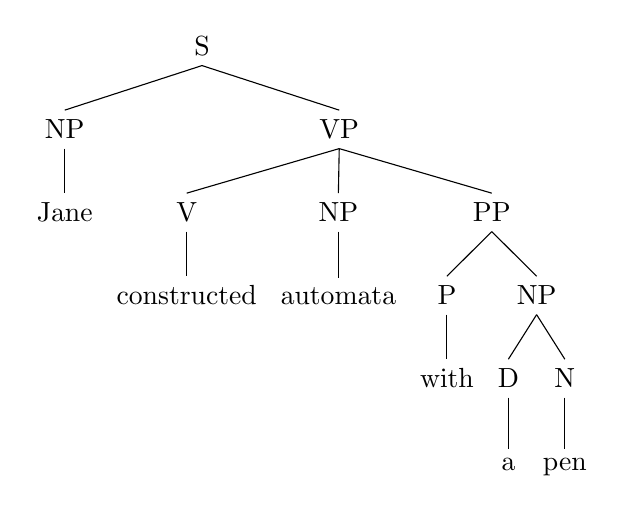
\begin{tikzpicture}[scale=1]
\Tree [.S [.NP Jane ] [.VP [.V constructed ] [.NP automata ] [.PP [.P with ] [.NP [.D a ] [.N pen ]] ] ] ]
\end{tikzpicture}
\\ \\
\begin{tikzpicture}[scale=1]
\Tree [.S [.NP ] [.VP [.V constructed ] [.NP [.N automata ] [.PP [.P with ] [.NP [.P with ] [.NP [.D a ] [.N pen ] ] ] ] ] ] ]
\end{tikzpicture}

\end{tcolorbox}

\paragraph{b)} my book in the man built a Jane by a pen \hfill \small{(4/20 pts)} \\

\begin{tcolorbox}
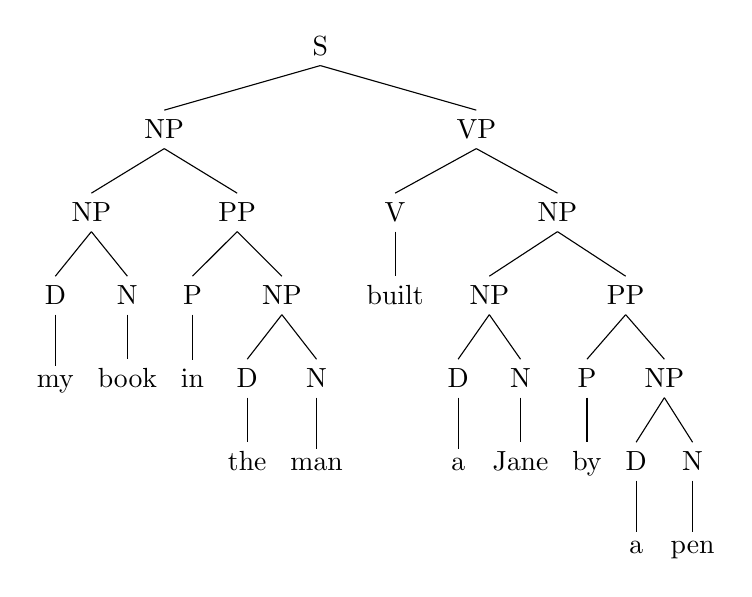
\begin{tikzpicture}[scale=1]
\Tree [.S [.NP [.NP [.D my ] [.N book ] ] [.PP [.P in ] [.NP [.D the ] [.N man ] ] ] ] [.VP [.V built ] [.NP [.NP [.D a ] [.N Jane ] ] [.PP [.P by ] [.NP [.D a ] [.N pen ] ] ] ] ]]
\end{tikzpicture}
\\ \\
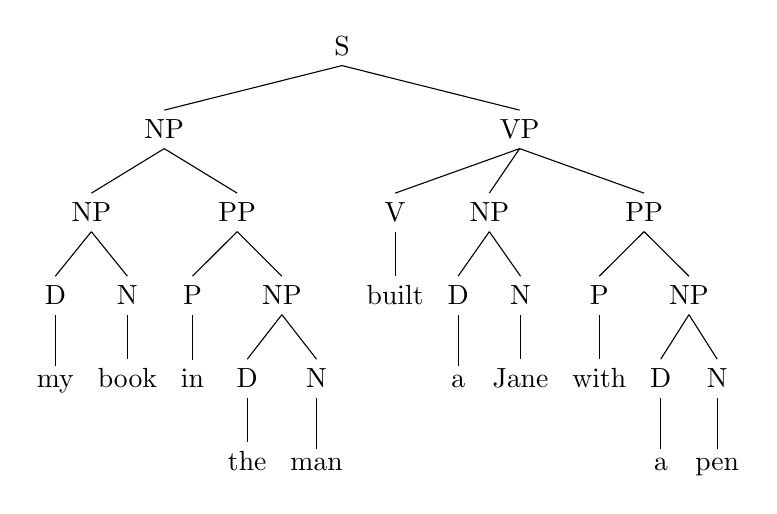
\begin{tikzpicture}[scale=1]
\Tree [.S [.NP [.NP [.D my ] [.N book ] ] [.PP [.P in ] [.NP [.D the ] [.N man ] ] ] ] [.VP [.V built ] [.NP [.D a ] [.N Jane ] ]  [.PP [.P with ] [.NP [.D a ] [.N pen ] ] ] ]  ]
\end{tikzpicture}
\end{tcolorbox}
\newpage

Given the CFG below, answer \textbf{c}, \textbf{d} and \textbf{e} \\

\begin{lstlisting}[style=output,mathescape=true]
S  $\to$ E
E  $\to$ E + T | E - T | T
T  $\to$ T * I | T / I | I
I  $\to$ 0 | 1 | 2 | 3 | 4 | 6 | 7 | 8 | 9
\end{lstlisting}

\paragraph{c)} Provide the left-most derivation of 7 - 4 * 3 step-by-step and plot the final parse \hfill \small{(4/20 pts)} \\
tree matching that derivation \\

\begin{tcolorbox}
The arrows means that the left most derivation. (I cannot put the L letter on to the top of the arrow.) \\
\vspace{2cm}
$S \rightarrow E \rightarrow E-T\rightarrow T - T \rightarrow I - T \rightarrow 7 - T \rightarrow 7 - T*I \rightarrow 7-I*I  \rightarrow 7 - 4 * I  \rightarrow 7-4*3$\\\\

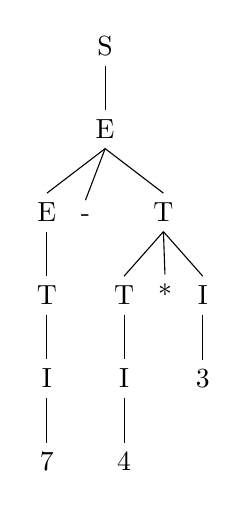
\begin{tikzpicture}[scale=1]

\Tree  [.S [.E [.E [.T [.I 7 ] ]  ] - [.T [.T [.I 4 ]  ] * [.I 3 ]  ] ]  ]

\end{tikzpicture}
\end{tcolorbox}

\paragraph{d)} Provide the right-most derivation of 7 - 4 * 3 step-by-step and plot the final parse \hfill \small{(4/20 pts)} \\
 tree matching that derivation \\
 
\begin{tcolorbox}
The arrows means that the right most derivation. (I cannot put the R letter on to the top of the arrow.) \\
\vspace{2cm}
$S \rightarrow E\rightarrow E-T\rightarrow E - T*I\rightarrow E-T*3 \rightarrow E - I*3 \rightarrow E- 4*3\rightarrow T - 4*3\rightarrow I-4*3 \rightarrow7-4*3$\\\\

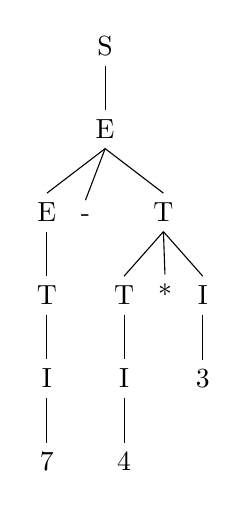
\begin{tikzpicture}[scale=1]

\Tree  [.S [.E [.E [.T [.I 7 ] ]  ] - [.T [.T [.I 4 ]  ] * [.I 3 ]  ] ]  ]

\end{tikzpicture}
\end{tcolorbox}


\paragraph{e)} Are the derivations in \textbf{c} and \textbf{d} in the same similarity class?  \hfill \small{(4/20 pts)} \\

\begin{tcolorbox}
Since the parse trees at the end of the derivations are same, we can say that the both of the parse trees are in the same similarity class. The parse trees are same because we change only the preference of the rules of the derivation and rules of the derivation are same in the both of the derivation of the parse trees.	
\end{tcolorbox}


\newpage
\section{Pushdown Automata \hfill \normalfont{(30 pts)}}

\paragraph{a)} 
Find the language recognized by the PDA given below \hfill \small{(5/30 pts)} \\

\begin{tikzpicture}[shorten >=1pt,node distance=3cm,on grid,auto]
\node[state,initial,initial text=] (q_0) {$q_0$};
\node[state] (q_1) [right=of q_0] {$q_1$};
\node[state] (q_2) [above right=of q_1] {$q_2$};
\node[state] (q_3) [below right=of q_1] {$q_3$};
\node[state,accepting](q_4) [right=of q_2] {$q_4$};
\node[state](q_5) [right=of q_3] {$q_5$};
\node[state,accepting](q_6) [right=of q_5] {$q_6$};
\path[->]

(q_0) edge node {$\varepsilon,\varepsilon \to \#$} (q_1)
(q_1) edge [loop below] node {$x,\varepsilon \to x$} (q_1)

%%
(q_1) edge node {$\varepsilon,\varepsilon \to \varepsilon$} (q_2)
(q_2) edge [loop above] node {$y,x \to \varepsilon$} (q_2)

(q_2) edge node {$\varepsilon,\# \to \varepsilon$} (q_4)
(q_4) edge [loop above] node {$z,\varepsilon \to \varepsilon$} (q_4)

%%%

(q_1) edge node {$\varepsilon,\varepsilon \to \varepsilon$} (q_3)
(q_3) edge [loop below] node {$y,\varepsilon \to \varepsilon$} (q_3)

(q_3) edge node {$\varepsilon,\varepsilon \to \varepsilon$} (q_5)
(q_5) edge [loop below] node {$z,x \to \varepsilon$} (q_5)

(q_5) edge node {$\varepsilon,\# \to \varepsilon$} (q_6)
;
\end{tikzpicture} \\

\begin{minipage}{0.60\textwidth}
where the transition $((q_i,\alpha,\beta),(q_j,\gamma)) $ is represented as: 
\end{minipage}
\begin{minipage}{0.30\textwidth}
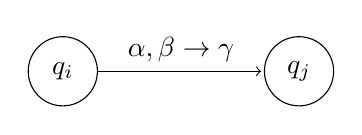
\begin{tikzpicture}[shorten >=1pt,node distance=3cm,on grid,auto]
\node[state] (q_i) {$q_i$};
\node[state] (q_j) [right=of q_i] {$q_j$};
\path[->]
(q_i) edge node {$\alpha,\beta \to \gamma$} (q_j);
\end{tikzpicture} \\
\end{minipage}


\begin{tcolorbox}
$\{x^i y^j z^k |$ i,j,k $\geq$ 0 and i = j or i=k $\}$
\end{tcolorbox}


\paragraph{b)} 
Design a PDA to recognize language $ L=\{x^n y^{m+n} x^m \mid \; n,m \geq 0; \; n,m \in \mathbb{N}  \} $  \hfill \small{(5/30 pts)} \\

\begin{tcolorbox}
\begin{center}
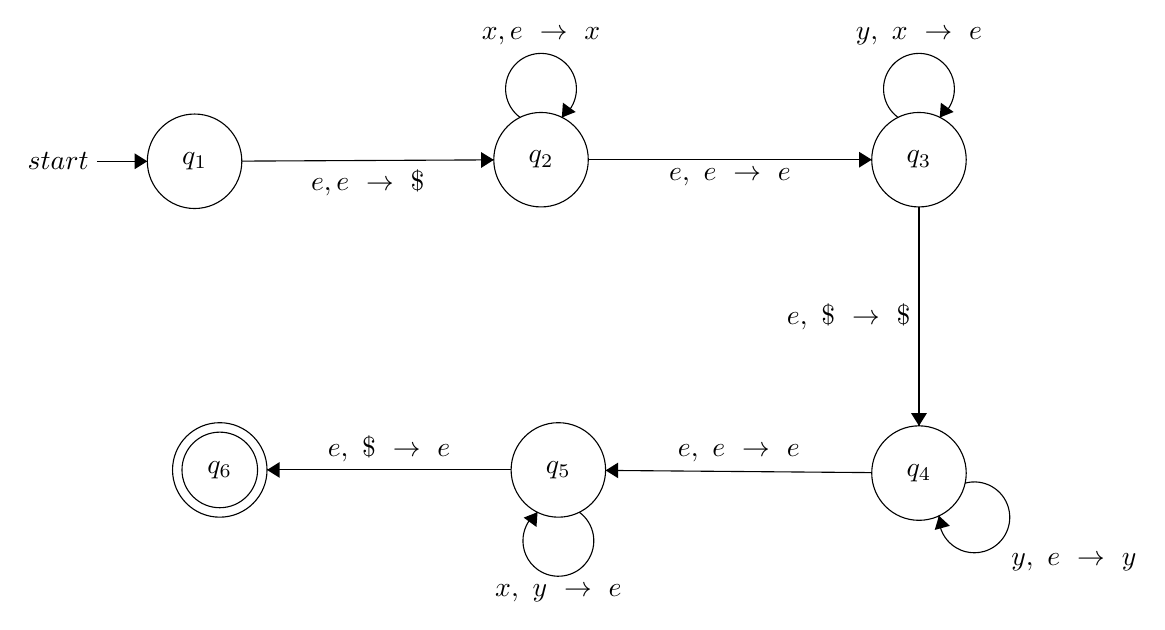
\begin{tikzpicture}[scale=0.2]
\tikzstyle{every node}+=[inner sep=0pt]
\draw [black] (34.4,-14.3) circle (3);
\draw (34.4,-14.3) node {$q_2$};
\draw [black] (58.4,-14.3) circle (3);
\draw (58.4,-14.3) node {$q_3$};
\draw [black] (58.4,-34.2) circle (3);
\draw (58.4,-34.2) node {$q_4$};
\draw [black] (35.5,-34) circle (3);
\draw (35.5,-34) node {$q_5$};
\draw [black] (14,-34) circle (3);
\draw (14,-34) node {$q_6$};
\draw [black] (14,-34) circle (2.4);
\draw [black] (12.4,-14.4) circle (3);
\draw (12.4,-14.4) node {$q_1$};
\draw [black] (33.077,-11.62) arc (234:-54:2.25);
\draw (34.4,-7.05) node [above] {$x,e\mbox{ }\rightarrow\mbox{ }x$};
\fill [black] (35.72,-11.62) -- (36.6,-11.27) -- (35.79,-10.68);
\draw [black] (37.4,-14.3) -- (55.4,-14.3);
\fill [black] (55.4,-14.3) -- (54.6,-13.8) -- (54.6,-14.8);
\draw (46.4,-14.8) node [below] {$e,\mbox{ }e\mbox{ }\rightarrow\mbox{ }e$};
\draw [black] (57.077,-11.62) arc (234:-54:2.25);
\draw (58.4,-7.05) node [above] {$y,\mbox{ }x\mbox{ }\rightarrow\mbox{ }e$};
\fill [black] (59.72,-11.62) -- (60.6,-11.27) -- (59.79,-10.68);
\draw [black] (58.4,-17.3) -- (58.4,-31.2);
\fill [black] (58.4,-31.2) -- (58.9,-30.4) -- (57.9,-30.4);
\draw (57.9,-24.25) node [left] {$e,\mbox{ }\$\mbox{ }\rightarrow\mbox{ }\$$};
\draw [black] (61.319,-34.841) arc (105.34019:-182.65981:2.25);
\draw (64.23,-39.84) node [right] {$y,\mbox{ }e\mbox{ }\rightarrow\mbox{ }y$};
\fill [black] (59.67,-36.91) -- (59.4,-37.81) -- (60.36,-37.55);
\draw [black] (55.4,-34.17) -- (38.5,-34.03);
\fill [black] (38.5,-34.03) -- (39.3,-34.53) -- (39.3,-33.53);
\draw (46.96,-33.54) node [above] {$e,\mbox{ }e\mbox{ }\rightarrow\mbox{ }e$};
\draw [black] (36.823,-36.68) arc (54:-234:2.25);
\draw (35.5,-41.25) node [below] {$x,\mbox{ }y\mbox{ }\rightarrow\mbox{ }e$};
\fill [black] (34.18,-36.68) -- (33.3,-37.03) -- (34.11,-37.62);
\draw [black] (32.5,-34) -- (17,-34);
\fill [black] (17,-34) -- (17.8,-34.5) -- (17.8,-33.5);
\draw (24.75,-33.5) node [above] {$e,\mbox{ }\$\mbox{ }\rightarrow\mbox{ }e$};
\draw [black] (15.4,-14.39) -- (31.4,-14.31);
\fill [black] (31.4,-14.31) -- (30.6,-13.82) -- (30.6,-14.82);
\draw (23.4,-14.88) node [below] {$e,e\mbox{ }\rightarrow\mbox{ }\$$};
\draw [black] (6.2,-14.4) -- (9.4,-14.4);
\draw (5.7,-14.4) node [left] {$start$};
\fill [black] (9.4,-14.4) -- (8.6,-13.9) -- (8.6,-14.9);
\end{tikzpicture}
\end{center}

\end{tcolorbox}

\newpage

\paragraph{c)} 
Design a PDA to recognize language $ L=\{x^n y^m \mid \; n < m \leq 2n; \; n,m \in \mathbb{N^+} \} $  \hfill \small{(10/30 pts)} \\
Do not use multi-symbol push/pop operations in your transitions. \\
Simulate the PDA on strings \textit{xxy} (with only one rejecting derivation) and \textit{xxyyyy} (accepting derivation) with transition tables. \\


\begin{tcolorbox}
CFG: $S \rightarrow xTyy$ \\ $T \rightarrow xTy | xTyy | e$  \\
PDA: \\ \\


\begin{center}
\begin{tikzpicture}[scale=0.2]
\tikzstyle{every node}+=[inner sep=0pt]
\draw [black] (7.9,-26.1) circle (3);
\draw (7.9,-26.1) node {$q_1$};
\draw [black] (27.3,-26.1) circle (3);
\draw (27.3,-26.1) node {$q_2$};
\draw [black] (46.6,-26.1) circle (3);
\draw (46.6,-26.1) node {$q_3$};
\draw [black] (46.6,-45.8) circle (3);
\draw (46.6,-45.8) node {$q_5$};
\draw [black] (46.6,-8.9) circle (3);
\draw (46.6,-8.9) node {$q_4$};
\draw [black] (46.6,-8.9) circle (2.4);
\draw [black] (10.9,-26.1) -- (24.3,-26.1);
\fill [black] (24.3,-26.1) -- (23.5,-25.6) -- (23.5,-26.6);
\draw (17.6,-26.6) node [below] {$e,e\mbox{ }\rightarrow\mbox{ }\$$};
\draw [black] (30.3,-26.1) -- (43.6,-26.1);
\fill [black] (43.6,-26.1) -- (42.8,-25.6) -- (42.8,-26.6);
\draw (36.95,-26.6) node [below] {$e,\mbox{ }e\mbox{ }\rightarrow\mbox{ }e$};
\draw [black] (25.977,-23.42) arc (234:-54:2.25);
\draw (27.3,-18.85) node [above] {$x,e\mbox{ }\rightarrow\mbox{ }x$};
\fill [black] (28.62,-23.42) -- (29.5,-23.07) -- (28.69,-22.48);
\draw [black] (45.138,-43.185) arc (-155.68563:-204.31437:17.571);
\fill [black] (45.14,-43.18) -- (45.26,-42.25) -- (44.35,-42.66);
\draw (43.08,-35.95) node [left] {$y,\mbox{ }x\mbox{ }\rightarrow\mbox{ }e$};
\draw [black] (47.573,-28.936) arc (15.62682:-15.62682:26.038);
\fill [black] (47.57,-28.94) -- (47.31,-29.84) -- (48.27,-29.57);
\draw (49.04,-35.95) node [right] {$y,\mbox{ }x\mbox{ }\rightarrow\mbox{ }x$};
\draw [black] (46.6,-23.1) -- (46.6,-11.9);
\fill [black] (46.6,-11.9) -- (46.1,-12.7) -- (47.1,-12.7);
\draw (47.1,-17.5) node [right] {$y,\mbox{ }\$\mbox{ }\rightarrow\mbox{ }e$};
\draw [black] (49.403,-25.065) arc (137.99099:-150.00901:2.25);
\draw (53.96,-26.9) node [right] {$y,x\mbox{ }\rightarrow\mbox{ }e$};
\fill [black] (49.13,-27.7) -- (49.39,-28.6) -- (50.06,-27.86);
\draw [black] (2.5,-26.1) -- (4.9,-26.1);
\draw (2,-26.1) node [left] {$start$};
\fill [black] (4.9,-26.1) -- (4.1,-25.6) -- (4.1,-26.6);
\end{tikzpicture}
\end{center}

Simulation of the string xxy \\\\\\\\\\\\\

\begin{table}[H]
\centering
\begin{tabular}{|l|l|l|l|}
\hline
Transition & Current State & Unread Input & Stack contents \\ \hline
1          & $q_1$         & xxy          & e              \\ \hline
2          & $q_2$         & xxy          & \$             \\ \hline
3          & $q_2$         & xy           & x\$            \\ \hline
4          & $q_2$         & y            & xx\$           \\ \hline
5          & $q_3$         & y            & xx\$           \\ \hline
6          & $q_3$         & e            & x\$            \\ \hline
\end{tabular}
\end{table}
Since at the end the stack is not empty and the state $q_3$ is not a accepting state, the string xxy will not be accepted. \\
Simulation of the string xxyyyy \\
\begin{table}[H]
\centering
\begin{tabular}{|l|l|l|l|}
\hline
Transition & Current State & Unread Input & Stack contents \\ \hline
1          & $q_1$         & xxyyyy       & e              \\ \hline
2          & $q_2$         & xxyyyy       & \$             \\ \hline
3          & $q_2$         & xyyyy        & x\$            \\ \hline
4          & $q_2$         & yyyy         & xx\$           \\ \hline
5          & $q_3$         & yyyy         & xx\$           \\ \hline
6          & $q_5$         & yyy          & x\$            \\ \hline
7          & $q_3$         & yy           & x\$            \\ \hline
8          & $q_3$         & y            & \$             \\ \hline
9          & $q_4$         & e            & e              \\ \hline
\end{tabular}
\end{table}
Since at the end the stack is empty and $q_4$ is accepting state, the string xxyyyy will be accepted. \\
\end{tcolorbox}

\paragraph{d)} Given two languages $L'$ and $L$ as $L'=\{w \mid \; w\in L; \; |w|=4n+2 \; for\; n\in \mathbb{N} \}$
\hfill \small{(10/30 pts)} \\
If $L$ is a CFL, show that $L'$ is also a CFL by constructing an automaton for $L'$ in terms of another automaton that recognizes $L$. \\


\begin{tcolorbox}
Denote L as L = $\{ K_L,\Sigma, \Gamma_L, \sigma_L,s_L,F_L\}$ where F is set of accepting states of the PDA L. \\
Define a DFA,say $L_0$, which recognizes the language $|w|=4n+2 \; for\; n\in \mathbb{N}$
as follows \\
\begin{center}
\begin{tikzpicture}[scale=0.2]
\tikzstyle{every node}+=[inner sep=0pt]
\draw [black] (10.4,-28.7) circle (3);
\draw (10.4,-28.7) node {$q_1$};
\draw [black] (27.4,-28.9) circle (3);
\draw (27.4,-28.9) node {$q_2$};
\draw [black] (54.4,-39.7) circle (3);
\draw (54.4,-39.7) node {$q_4$};
\draw [black] (65.2,-29.8) circle (3);
\draw (65.2,-29.8) node {$q_5$};
\draw [black] (52.9,-18.9) circle (3);
\draw (52.9,-18.9) node {$q_6$};
\draw [black] (42.8,-28.9) circle (3);
\draw (42.8,-28.9) node {$q_3$};
\draw [black] (42.8,-28.9) circle (2.4);
\draw [black] (5.3,-28.7) -- (7.4,-28.7);
\draw (4.8,-28.7) node [left] {$start$};
\fill [black] (7.4,-28.7) -- (6.6,-28.2) -- (6.6,-29.2);
\draw [black] (13.4,-28.74) -- (24.4,-28.86);
\fill [black] (24.4,-28.86) -- (23.61,-28.36) -- (23.59,-29.36);
\draw (18.9,-29.31) node [below] {$\Sigma$};
\draw [black] (30.4,-28.9) -- (39.8,-28.9);
\fill [black] (39.8,-28.9) -- (39,-28.4) -- (39,-29.4);
\draw (35.1,-29.4) node [below] {$\Sigma$};
\draw [black] (45,-30.94) -- (52.2,-37.66);
\fill [black] (52.2,-37.66) -- (51.96,-36.74) -- (51.28,-37.48);
\draw (47.5,-34.78) node [below] {$\Sigma$};
\draw [black] (56.61,-37.67) -- (62.99,-31.83);
\fill [black] (62.99,-31.83) -- (62.06,-32) -- (62.74,-32.74);
\draw (60.9,-35.24) node [below] {$\Sigma$};
\draw [black] (62.95,-27.81) -- (55.15,-20.89);
\fill [black] (55.15,-20.89) -- (55.41,-21.79) -- (56.08,-21.05);
\draw (60.14,-23.86) node [above] {$\Sigma$};
\draw [black] (50.77,-21.01) -- (44.93,-26.79);
\fill [black] (44.93,-26.79) -- (45.85,-26.58) -- (45.15,-25.87);
\draw (46.75,-23.42) node [above] {$\Sigma$};
\end{tikzpicture}
\end{center}

Then, we can say that $|w|=4n+2 \; for\; n\in \mathbb{N}$,say $L_0$, is regular language. Since L' is intersection of the L and  $L_0$, it is context free language.
I will give the proof by using book's proof.
We have two machines one is PDA L=$(K_L,\Sigma, \Gamma_L, \sigma_L,s_L,F_L)$ and the other one is DFA $L_0$ = $(K_0,\Sigma, \sigma_0,s_0,F_0)$. The idea is combining these two automatons into single pushdown automaton M that carries out computations by $L$ and $L_0$ in parallel and accepts only if both of the automatons would accepted. We can specify M = $(K,\Sigma,\Gamma,\sigma,s,F)$ where \\ $K = K_LxK_0$ \\ $\Gamma = \Gamma_L$ \\ $s = (s_Lxs_0)$ \\ $F = F_LxF_0$ \\ \\
$\sigma$, the transition function of the automaton M, is defined as follows. For each transition of the pushdown automaton L $((q_1,a,\beta ),(p_1,\gamma )) \in  \sigma_L $, and for each state $q_2 \in K_0 $, we add to $ \sigma $ the transition $(((q_1,q_2)a,\beta),((p_1,\sigma_0(q_2,a)),\gamma ))$; and for each transtion of the form $((q_1,e,\beta),(p_1,\gamma)) \in \sigma_L$ and each state $q_2 \in K_0$, we add the transition $(((q_1,q_2),e,\beta),((q_1,q_2),\gamma))$. That means that M passes from state $(q_1,q_2)$ to state $(p_1,p_2)$ in the same way that $M_1$ passes from state $q_1$ to $p_1$, except that in addition M keeps track of the change in the state of $L_0$ caused by reading the same input. 

\end{tcolorbox}






\newpage
\section{Closure Properties \hfill \normalfont{(20 pts)}}

Let $L_1$ and $L_2$ be context-free languages which are not regular, and let $L_3$ be a regular language. Determine whether the following languages are necessarily CFLs or not. If they need to be context-free, explain your reasoning. If not, give one example where the language is a CFL and a counter example where the language is not a CFL. \\

\paragraph{a)} $L_4 = L_1 \cap (L_2 \setminus L_3)$ \hfill \small{(10/20 pts)} \\

\begin{tcolorbox}
We can write $(L_2 \setminus L_3) $ as $L_2 \cap \overline{L_3}$ and $L_2 \cap \overline{L_3}$ is context free because $\overline{L_3}$ is regular since regular languages are closed under complementation and intersection of a regular language and context free language is context free by the theorem (3.5.2). Then, since both of the languages that $L_1$ and $L_2 \cap \overline{L_3}$ are both context free and context free language are not closed under the intersection with each other, $L_4$ is not necessarily context free language. \\ For example, take $L_1 = \{ a^nb^nc^m | n \geq 0 and m \geq 0\}$ and $L_2 = \{a^mb^nc^n | n \geq 0 and m \geq 0  \}$. Then, $L_3 = L_1 \cap L_2 = \{a^nb^nc^n | n \geq 0\}$ is not context free because $L_1$ says that the number of a's should be equal to the number of b's and $L_2$ says that the number b's should be equal to the number of c's. However, in their intersections $L_3$, both conditions need not to be true for satisfying the property of $L_3$. But a pushdown automata can compare only two. Therefore, $L_3$ is not context free language since it cannot be recognized by a pushdown automata.
\end{tcolorbox}

\paragraph{b)} $L_5 = (L_1 \cap L_3)\text{*}$ \hfill \small{(10/20 pts)} \\

\begin{tcolorbox}
The intersection of a context free language and regular language is a context free language. It is clear by the theorem from the book whose number is (3.5.2). Since ($L_1 \cap L_3$) is context free language clarified with theorem 3.5.2 and every context free language are closed under Kleene star operation by theorem from the book whose number is (3.5.1), we can say that $L_5$ is context free language.
\end{tcolorbox}





\newpage
\section{Pumping Theorem \hfill \normalfont{(20 pts)}}

\paragraph{a)} Show that $L=\{a^n m^n t^i \mid \; n\leq i \leq 2n\}$ is not a Context Free Language \hfill \small{(10/20 pts)} \\
using Pumping Theorem for CFLs. \\

\begin{tcolorbox}
We state by using pumping lemma that for every context free language, there is an integer called pumping length such that for every string which is element of L, context free language, the length of the string is greater than or equal to the pumping length n and we can parse that string,say s, as s = uvxyz where $|vy| \geq 0$ which means that both of the v and y subtrings cannot be empty and $|vxy| \leq n$ and for every positive integer, say i=0,1,2,3,..., the string $uv^ixy^iz$ must be in the language. \\
Take the string $a^nb^nt^n$. Since the property of the language is satisfied the string is in the language L.Since the length of the substring vxy is less than or equal to the pumping length n and and between a and t there are m letters of n times, it cannot contain more than two symbols. If we analyze the cases, there are four cases as follows: \\
a)vxy contains only m's, it cannot be in the language since it contains more m's than a's. \\
b)vxy contains only a's, it cannot be in the language since it contains more a's than m's. \\
c)vxy contains m's and t's, it cannot be in the language since it contains more m's than a's.
d)vxy contains a's and m's, it cannot be in the language since it contains less t's than a's and m's. \\

Since we examine all of the cases and one of the cases must be true eventually, the string cannot be in the language in any case. Therefore, the language $L=\{a^n m^n t^i \mid \; n\leq i \leq 2n\}$ is not context free language.
\end{tcolorbox}


\paragraph{b)} Show that $L=\{a^n b^{2n} a^n \mid \; n \in \mathbb{N+} \}$ is not a Context Free Language \hfill \small{(10/20 pts)} \\
using Pumping Theorem for CFLs. \\

\begin{tcolorbox}
We state by using pumping lemma that for every context free language, there is an integer called pumping length such that for every string which is element of L, context free language, the length of the string is greater than or equal to the pumping length n and we can parse that string,say s, as s = uvxyz where $|vy| \geq 0$ which means that both of the v and y subtrings cannot be empty and $|vxy| \leq n$ and for every positive integer, say i=0,1,2,3,..., the string $uv^ixy^iz$ must be in the language. \\
Take the string $a^nb^{2n}a^n$. Since the property of the language is satisfied the string is in the language L. Since the length of the substring vxy is less than or equal to the pumping length n, vxy substring can only contain a's or b's or a's before b's or b's before a's.($a^p$,$b^{2p}$,$a^p$ not from all three). If we analyze the cases, there are five cases as follows: \\
a)vxy contains only b's, it cannot be in the language since it does not contain b's exactly two times of a's from the first part of the string and a's from the last part of the string. \\
b)vxy contains only a's from the first part of the substring, it cannot be in the language since it contains more a's in the first part of the substring than last part of the substring. \\
c)vxy contains only a's from the last part of the substring, it cannot be in the language since it contains more a's in the last part of the substring than first part of the substring. \\
d)vxy contains b's and a's from the last part of the substring, it cannot be in the language since it cannot be in the language since it contains more a's in the last part of the substring than first part of the substring. \\
e)vxy contains a's from the first part of the substring and b's , it cannot be in the language since it cannot be in the language since it contains more a's in the first part of the substring than last part of the substring. \\

Since we examine all of the cases and one of the cases must be true eventually, the string cannot be in the language in any case. Therefore, the language $L=\{a^n b^{2n} a^n \mid \; n \in \mathbb{N+} \}$ is not context free language.
\end{tcolorbox}





\newpage
\section{CNF and CYK \hfill \normalfont{(not graded)}}

\paragraph{a)} Convert the given context-free grammar to Chomsky Normal Form. \\

$ S   \to XSX \mid xY $ \\
$ X   \to Y \mid S $ \\
$ Y   \to z \mid \varepsilon $ \\

\begin{tcolorbox}
answer here ...
\vspace{18cm} % remove this after your answer
\end{tcolorbox}


\paragraph{b)} Use the grammar below to parse the given sentence using Cocke–Younger–Kasami algorithm. \\
Plot the parse trees. \\

\begin{multicols}{2}
S $\to$ NP VP \\
S $\to$ X1 VP \\
X1 $\to$ Aux NP \\
S $\to$ book $\mid$ include $\mid$ prefer \\
S $\to$ Verb NP \\
S $\to$ X2 PP \\
S $\to$ Verb PP \\
S $\to$ VP PP \\
NP $\to$ I $\mid$ she $\mid$ me $\mid$ Houston \\
NP $\to$ Det Nom \\
Nom $\to$ book $\mid$ flight $\mid$ meal $\mid$ money \\
Nom $\to$ Nom Noun \\
Nom $\to$ Nom PP \\
VP $\to$ book $\mid$ include $\mid$ prefer \\
VP $\to$ Verb NP \\
VP $\to$ X2 PP \\
X2 $\to$ Verb NP \\
VP $\to$ Verb PP \\
VP $\to$ VP PP \\
PP $\to$ Prep NP \\
Det $\to$ that $\mid$ this $\mid$ the $\mid$ a \\
Noun $\to$ book $\mid$ flight $\mid$ meal $\mid$ money \\
Verb $\to$ book $\mid$ include $\mid$ prefer \\
Aux $\to$ does \\
Prep $\to$ from $\mid$ to $\mid$ on $\mid$ near $\mid$ through \\
\end{multicols}

\vspace{5mm}

book the flight through Houston \\

\begin{tcolorbox}

\scriptsize

Empty parse table:\\
\begin{tikzpicture}[node distance=0cm, outer sep = 0pt]

\node[terminal] (l0) {
    \begin{tabular}{@{}P{2.9cm}|@{}P{2.9cm}|@{}P{2.9cm}|@{}P{2.9cm}|@{}P{2.9cm}}
    book & the & flight & through & Houston \\
    \end{tabular}
};

\node[nonterminal] (l1) [above = of l0] {
    \begin{tabular}{@{}P{2.9cm}|@{}P{2.9cm}|@{}P{2.9cm}|@{}P{2.9cm}|@{}P{2.9cm}}
    1:1 & 
    2:2 & 
    3:3 & 
    4:4 & 
    5:5 \\
    \end{tabular}
};

\node[nonterminal] (l2) [above = of l1.north] {
    \begin{tabular}{@{}P{2.9cm}|@{}P{2.9cm}|@{}P{2.9cm}|@{}P{2.9cm}}
    1:2 $\to$ 1:1 2:2 & 
    2:3 $\to$ 2:2 3:3 & 
    3:4 $\to$ 3:3 4:4 & 
    4:5 $\to$ 4:4 5:5 \\
    \end{tabular}
};

\node[nonterminal] (l3) [above = of l2.north] {
    \begin{tabular}{@{}P{2.9cm}|@{}P{2.9cm}|@{}P{2.9cm}}
        \begin{tabular}{@{}l} 1:3 $\to$ 1:1 2:3 \\ 1:3 $\to$ 1:2 3:3 \end{tabular}& 
        \begin{tabular}{@{}l} 2:4 $\to$ 2:2 3:4 \\ 2:4 $\to$ 2:3 4:4 \end{tabular}& 
        \begin{tabular}{@{}l} 3:5 $\to$ 3:3 4:5 \\ 3:5 $\to$ 3:4 5:5 \end{tabular}\\
    \end{tabular}
};

\node[nonterminal] (l4) [above = of l3.north] {
    \begin{tabular}{@{}P{2.9cm}|@{}P{2.9cm}}
        \begin{tabular}{@{}l}1:4 $\to$ 1:1 2:4 \\ 1:4 $\to$ 1:2 3:4 \\ 1:4 $\to$ 1:3 4:4 \end{tabular}& 
        \begin{tabular}{@{}l}2:5 $\to$ 2:2 3:5 \\ 2:5 $\to$ 2:3 4:5 \\ 2:5 $\to$ 2:4 5:5 \end{tabular}\\
    \end{tabular}
};

\node[nonterminal] (l5) [above = of l4.north] {
    \begin{tabular}{@{}P{2.9cm}}
        \begin{tabular}{@{}l}
        1:5 $\to$ 1:1 2:5 \\ 1:5 $\to$ 1:2 3:5 \\ 
        1:5 $\to$ 1:3 4:5 \\ 1:5 $\to$ 1:4 5:5 
        \end{tabular}\\
    \end{tabular}
};

\end{tikzpicture}\\\\

rest of the answer here ...\\
\vspace{4cm} % remove this after your answer
\end{tcolorbox}



\newpage
\section{Deterministic Pushdown Automata \hfill \normalfont{(not graded)}}
Provide a DPDA to recognize the given languages, the DPDA must read its entire input and finish with an empty stack.
\paragraph{a)} $a^*bc \cup a^nb^nc$ \\

\begin{tcolorbox}
answer here ...
\vspace{12cm} % remove this after your answer
\end{tcolorbox}

\newpage

\paragraph{b)} $(aa)^*c \cup a^nb^nc$ \\

\begin{tcolorbox}
answer here ...
\vspace{12cm} % remove this after your answer
\end{tcolorbox}



\end{document}

​
